\documentclass[tikz,border=10pt]{standalone}
\usepackage{tikz}
\usepackage{tikz-cd}
\usetikzlibrary{arrows,automata,shapes,positioning,decorations.pathmorphing}
% \tikzset{->,>=stealth',auto}
\tikzset{->,auto}
\tikzset{>={Latex[width=2mm,length=2mm]}}
\tikzset{state with output/.style={shape=rectangle split, rectangle
    split parts=2, draw, fill=white,
    initial text=, inner sep=1mm}}
\tikzset{every node={font=\footnotesize}}
\begin{document}
  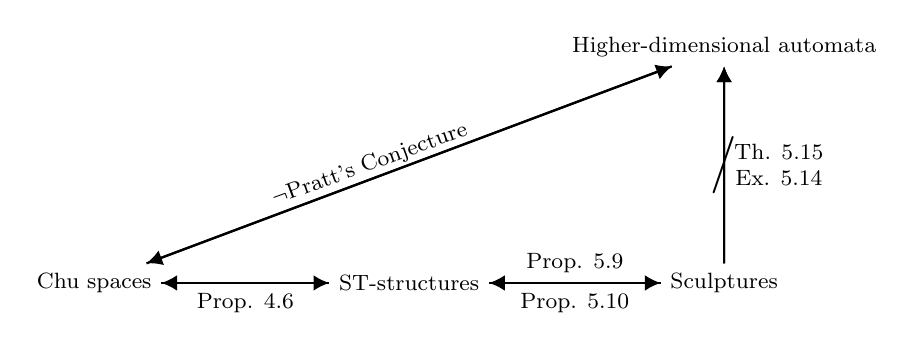
\begin{tikzpicture}[node distance=4cm, align=center]
  \tikzstyle{every node}=[font=\footnotesize]
    \tikzstyle{every state}=[fill=white,shape=circle,inner sep=.5mm,minimum size=3mm]
    \title{Diagram}
    
    \node(q1) []                {Chu spaces};
    \node(q2) [right of=q1]     {ST-structures};
    \node(q3) [right of=q2]     {Sculptures};
    \node(q4) at (8,3) []     {Higher-dimensional automata};
    %\node(q5) at (4,1.5) {\huge $\times$};
    \node(q5) at (8,1.5) {\huge /};
    \node[rotate=20](q6) at (3.5,1.5) {$\neg$Pratt's Conjecture};
    
    \draw [->][draw=black, thick] (q1) to node [above] {} (q2);
    \draw [->][draw=black, thick] (q2) to node [below] {Prop. 4.6} (q1);
    \draw [->][draw=black, thick] (q2) to node [above] {Prop. 5.9} (q3);
    \draw [->][draw=black, thick] (q3) to node [below] {Prop. 5.10} (q2);
    %\draw [->][draw=black, thick] (q3) to node [above right] {Def. 5.13} (q4);
    \draw [->][draw=black, thick] (q3) to node [right] {Th. 5.15 \\ Ex. 5.14} (q4);
    \draw [->][draw=black, thick] (q3) to node [] {} (q4);
    \draw [->][draw=black, thick] (q1) to node [above left] {} (q4);
    \draw [->][draw=black, thick] (q4) to node [above left] {} (q1);

  \end{tikzpicture}
\end{document}